\documentclass[11pt]{article}
% NOTE: Add in the relevant information to the commands below; or, if you'll be using the same information frequently, add these commands at the top of paolo-pset.tex file. 
\newcommand{\name}{Agustin Esteva}
\newcommand{\email}{aesteva@uchicago.edu}
\newcommand{\classnum}{207}
\newcommand{\subject}{Honors Analysis in $\bbR^n$}
\newcommand{\instructors}{Luis Silvestre}
\newcommand{\assignment}{Problem Set 6}
\newcommand{\semester}{Fall 2024}
\newcommand{\duedate}{2024-11-11}
\newcommand{\bA}{\mathbf{A}}
\newcommand{\bB}{\mathbf{B}}
\newcommand{\bC}{\mathbf{C}}
\newcommand{\bD}{\mathbf{D}}
\newcommand{\bE}{\mathbf{E}}
\newcommand{\bF}{\mathbf{F}}
\newcommand{\bG}{\mathbf{G}}
\newcommand{\bH}{\mathbf{H}}
\newcommand{\bI}{\mathbf{I}}
\newcommand{\bJ}{\mathbf{J}}
\newcommand{\bK}{\mathbf{K}}
\newcommand{\bL}{\mathbf{L}}
\newcommand{\bM}{\mathbf{M}}
\newcommand{\bN}{\mathbf{N}}
\newcommand{\bO}{\mathbf{O}}
\newcommand{\bP}{\mathbf{P}}
\newcommand{\bQ}{\mathbf{Q}}
\newcommand{\bR}{\mathbf{R}}
\newcommand{\bS}{\mathbf{S}}
\newcommand{\bT}{\mathbf{T}}
\newcommand{\bU}{\mathbf{U}}
\newcommand{\bV}{\mathbf{V}}
\newcommand{\bW}{\mathbf{W}}
\newcommand{\bX}{\mathbf{X}}
\newcommand{\bY}{\mathbf{Y}}
\newcommand{\bZ}{\mathbf{Z}}

%% blackboard bold math capitals
\newcommand{\bbA}{\mathbb{A}}
\newcommand{\bbB}{\mathbb{B}}
\newcommand{\bbC}{\mathbb{C}}
\newcommand{\bbD}{\mathbb{D}}
\newcommand{\bbE}{\mathbb{E}}
\newcommand{\bbF}{\mathbb{F}}
\newcommand{\bbG}{\mathbb{G}}
\newcommand{\bbH}{\mathbb{H}}
\newcommand{\bbI}{\mathbb{I}}
\newcommand{\bbJ}{\mathbb{J}}
\newcommand{\bbK}{\mathbb{K}}
\newcommand{\bbL}{\mathbb{L}}
\newcommand{\bbM}{\mathbb{M}}
\newcommand{\bbN}{\mathbb{N}}
\newcommand{\bbO}{\mathbb{O}}
\newcommand{\bbP}{\mathbb{P}}
\newcommand{\bbQ}{\mathbb{Q}}
\newcommand{\bbR}{\mathbb{R}}
\newcommand{\bbS}{\mathbb{S}}
\newcommand{\bbT}{\mathbb{T}}
\newcommand{\bbU}{\mathbb{U}}
\newcommand{\bbV}{\mathbb{V}}
\newcommand{\bbW}{\mathbb{W}}
\newcommand{\bbX}{\mathbb{X}}
\newcommand{\bbY}{\mathbb{Y}}
\newcommand{\bbZ}{\mathbb{Z}}

%% script math capitals
\newcommand{\sA}{\mathscr{A}}
\newcommand{\sB}{\mathscr{B}}
\newcommand{\sC}{\mathscr{C}}
\newcommand{\sD}{\mathscr{D}}
\newcommand{\sE}{\mathscr{E}}
\newcommand{\sF}{\mathscr{F}}
\newcommand{\sG}{\mathscr{G}}
\newcommand{\sH}{\mathscr{H}}
\newcommand{\sI}{\mathscr{I}}
\newcommand{\sJ}{\mathscr{J}}
\newcommand{\sK}{\mathscr{K}}
\newcommand{\sL}{\mathscr{L}}
\newcommand{\sM}{\mathscr{M}}
\newcommand{\sN}{\mathscr{N}}
\newcommand{\sO}{\mathscr{O}}
\newcommand{\sP}{\mathscr{P}}
\newcommand{\sQ}{\mathscr{Q}}
\newcommand{\sR}{\mathscr{R}}
\newcommand{\sS}{\mathscr{S}}
\newcommand{\sT}{\mathscr{T}}
\newcommand{\sU}{\mathscr{U}}
\newcommand{\sV}{\mathscr{V}}
\newcommand{\sW}{\mathscr{W}}
\newcommand{\sX}{\mathscr{X}}
\newcommand{\sY}{\mathscr{Y}}
\newcommand{\sZ}{\mathscr{Z}}
\newcommand{\osc}{\text{osc}}
\newcommand{\diam}{\text{diam}}


\renewcommand{\emptyset}{\O}

\newcommand{\abs}[1]{\lvert #1 \rvert}
\newcommand{\norm}[1]{\lVert #1 \rVert}
\newcommand{\sm}{\setminus}
\usepackage{tikz}
\usepackage{pgfplots}
\pgfplotsset{compat=1.18}


\newcommand{\sarr}{\rightarrow}
\newcommand{\arr}{\longrightarrow}

% NOTE: Defining collaborators is optional; to not list collaborators, comment out the line below.
%\newcommand{\collaborators}{Alyssa P. Hacker (\texttt{aphacker}), Ben Bitdiddle (\texttt{bitdiddle})}

% Copyright 2021 Paolo Adajar (padajar.com, paoloadajar@mit.edu)
% 
% Permission is hereby granted, free of charge, to any person obtaining a copy of this software and associated documentation files (the "Software"), to deal in the Software without restriction, including without limitation the rights to use, copy, modify, merge, publish, distribute, sublicense, and/or sell copies of the Software, and to permit persons to whom the Software is furnished to do so, subject to the following conditions:
%
% The above copyright notice and this permission notice shall be included in all copies or substantial portions of the Software.
% 
% THE SOFTWARE IS PROVIDED "AS IS", WITHOUT WARRANTY OF ANY KIND, EXPRESS OR IMPLIED, INCLUDING BUT NOT LIMITED TO THE WARRANTIES OF MERCHANTABILITY, FITNESS FOR A PARTICULAR PURPOSE AND NONINFRINGEMENT. IN NO EVENT SHALL THE AUTHORS OR COPYRIGHT HOLDERS BE LIABLE FOR ANY CLAIM, DAMAGES OR OTHER LIABILITY, WHETHER IN AN ACTION OF CONTRACT, TORT OR OTHERWISE, ARISING FROM, OUT OF OR IN CONNECTION WITH THE SOFTWARE OR THE USE OR OTHER DEALINGS IN THE SOFTWARE.

\usepackage{fullpage}
\usepackage{enumitem}
\usepackage{amsfonts, amssymb, amsmath,amsthm}
\usepackage{mathtools}
\usepackage[pdftex, pdfauthor={\name}, pdftitle={\classnum~\assignment}]{hyperref}
\usepackage[dvipsnames]{xcolor}
\usepackage{bbm}
\usepackage{graphicx}
\usepackage{mathrsfs}
\usepackage{pdfpages}
\usepackage{tabularx}
\usepackage{pdflscape}
\usepackage{makecell}
\usepackage{booktabs}
\usepackage{natbib}
\usepackage{caption}
\usepackage{subcaption}
\usepackage{physics}
\usepackage[many]{tcolorbox}
\usepackage{version}
\usepackage{ifthen}
\usepackage{cancel}
\usepackage{listings}
\usepackage{courier}

\usepackage{tikz}
\usepackage{istgame}

\hypersetup{
	colorlinks=true,
	linkcolor=blue,
	filecolor=magenta,
	urlcolor=blue,
}

\setlength{\parindent}{0mm}
\setlength{\parskip}{2mm}

\setlist[enumerate]{label=({\alph*})}
\setlist[enumerate, 2]{label=({\roman*})}

\allowdisplaybreaks[1]

\newcommand{\psetheader}{
	\ifthenelse{\isundefined{\collaborators}}{
		\begin{center}
			{\setlength{\parindent}{0cm} \setlength{\parskip}{0mm}
				
				{\textbf{\classnum~\semester:~\assignment} \hfill \name}
				
				\subject \hfill \href{mailto:\email}{\tt \email}
				
				Instructor(s):~\instructors \hfill Due Date:~\duedate	
				
				\hrulefill}
		\end{center}
	}{
		\begin{center}
			{\setlength{\parindent}{0cm} \setlength{\parskip}{0mm}
				
				{\textbf{\classnum~\semester:~\assignment} \hfill \name\footnote{Collaborator(s): \collaborators}}
				
				\subject \hfill \href{mailto:\email}{\tt \email}
				
				Instructor(s):~\instructors \hfill Due Date:~\duedate	
				
				\hrulefill}
		\end{center}
	}
}

\renewcommand{\thepage}{\classnum~\assignment \hfill \arabic{page}}

\makeatletter
\def\points{\@ifnextchar[{\@with}{\@without}}
\def\@with[#1]#2{{\ifthenelse{\equal{#2}{1}}{{[1 point, #1]}}{{[#2 points, #1]}}}}
\def\@without#1{\ifthenelse{\equal{#1}{1}}{{[1 point]}}{{[#1 points]}}}
\makeatother

\newtheoremstyle{theorem-custom}%
{}{}%
{}{}%
{\itshape}{.}%
{ }%
{\thmname{#1}\thmnumber{ #2}\thmnote{ (#3)}}

\theoremstyle{theorem-custom}

\newtheorem{theorem}{Theorem}
\newtheorem{lemma}[theorem]{Lemma}
\newtheorem{example}[theorem]{Example}

\newenvironment{problem}[1]{\color{black} #1}{}

\newenvironment{solution}{%
	\leavevmode\begin{tcolorbox}[breakable, colback=green!5!white,colframe=green!75!black, enhanced jigsaw] \proof[\scshape Solution:] \setlength{\parskip}{2mm}%
	}{\renewcommand{\qedsymbol}{$\blacksquare$} \endproof \end{tcolorbox}}

\newenvironment{reflection}{\begin{tcolorbox}[breakable, colback=black!8!white,colframe=black!60!white, enhanced jigsaw, parbox = false]\textsc{Reflections:}}{\end{tcolorbox}}

\newcommand{\qedh}{\renewcommand{\qedsymbol}{$\blacksquare$}\qedhere}

\definecolor{mygreen}{rgb}{0,0.6,0}
\definecolor{mygray}{rgb}{0.5,0.5,0.5}
\definecolor{mymauve}{rgb}{0.58,0,0.82}

% from https://github.com/satejsoman/stata-lstlisting
% language definition
\lstdefinelanguage{Stata}{
	% System commands
	morekeywords=[1]{regress, reg, summarize, sum, display, di, generate, gen, bysort, use, import, delimited, predict, quietly, probit, margins, test},
	% Reserved words
	morekeywords=[2]{aggregate, array, boolean, break, byte, case, catch, class, colvector, complex, const, continue, default, delegate, delete, do, double, else, eltypedef, end, enum, explicit, export, external, float, for, friend, function, global, goto, if, inline, int, local, long, mata, matrix, namespace, new, numeric, NULL, operator, orgtypedef, pointer, polymorphic, pragma, private, protected, public, quad, real, return, rowvector, scalar, short, signed, static, strL, string, struct, super, switch, template, this, throw, transmorphic, try, typedef, typename, union, unsigned, using, vector, version, virtual, void, volatile, while,},
	% Keywords
	morekeywords=[3]{forvalues, foreach, set},
	% Date and time functions
	morekeywords=[4]{bofd, Cdhms, Chms, Clock, clock, Cmdyhms, Cofc, cofC, Cofd, cofd, daily, date, day, dhms, dofb, dofC, dofc, dofh, dofm, dofq, dofw, dofy, dow, doy, halfyear, halfyearly, hh, hhC, hms, hofd, hours, mdy, mdyhms, minutes, mm, mmC, mofd, month, monthly, msofhours, msofminutes, msofseconds, qofd, quarter, quarterly, seconds, ss, ssC, tC, tc, td, th, tm, tq, tw, week, weekly, wofd, year, yearly, yh, ym, yofd, yq, yw,},
	% Mathematical functions
	morekeywords=[5]{abs, ceil, cloglog, comb, digamma, exp, expm1, floor, int, invcloglog, invlogit, ln, ln1m, ln, ln1p, ln, lnfactorial, lngamma, log, log10, log1m, log1p, logit, max, min, mod, reldif, round, sign, sqrt, sum, trigamma, trunc,},
	% Matrix functions
	morekeywords=[6]{cholesky, coleqnumb, colnfreeparms, colnumb, colsof, corr, det, diag, diag0cnt, el, get, hadamard, I, inv, invsym, issymmetric, J, matmissing, matuniform, mreldif, nullmat, roweqnumb, rownfreeparms, rownumb, rowsof, sweep, trace, vec, vecdiag, },
	% Programming functions
	morekeywords=[7]{autocode, byteorder, c, _caller, chop, abs, clip, cond, e, fileexists, fileread, filereaderror, filewrite, float, fmtwidth, has_eprop, inlist, inrange, irecode, matrix, maxbyte, maxdouble, maxfloat, maxint, maxlong, mi, minbyte, mindouble, minfloat, minint, minlong, missing, r, recode, replay, return, s, scalar, smallestdouble,},
	% Random-number functions
	morekeywords=[8]{rbeta, rbinomial, rcauchy, rchi2, rexponential, rgamma, rhypergeometric, rigaussian, rlaplace, rlogistic, rnbinomial, rnormal, rpoisson, rt, runiform, runiformint, rweibull, rweibullph,},
	% Selecting time-span functions
	morekeywords=[9]{tin, twithin,},
	% Statistical functions
	morekeywords=[10]{betaden, binomial, binomialp, binomialtail, binormal, cauchy, cauchyden, cauchytail, chi2, chi2den, chi2tail, dgammapda, dgammapdada, dgammapdadx, dgammapdx, dgammapdxdx, dunnettprob, exponential, exponentialden, exponentialtail, F, Fden, Ftail, gammaden, gammap, gammaptail, hypergeometric, hypergeometricp, ibeta, ibetatail, igaussian, igaussianden, igaussiantail, invbinomial, invbinomialtail, invcauchy, invcauchytail, invchi2, invchi2tail, invdunnettprob, invexponential, invexponentialtail, invF, invFtail, invgammap, invgammaptail, invibeta, invibetatail, invigaussian, invigaussiantail, invlaplace, invlaplacetail, invlogistic, invlogistictail, invnbinomial, invnbinomialtail, invnchi2, invnF, invnFtail, invnibeta, invnormal, invnt, invnttail, invpoisson, invpoissontail, invt, invttail, invtukeyprob, invweibull, invweibullph, invweibullphtail, invweibulltail, laplace, laplaceden, laplacetail, lncauchyden, lnigammaden, lnigaussianden, lniwishartden, lnlaplaceden, lnmvnormalden, lnnormal, lnnormalden, lnwishartden, logistic, logisticden, logistictail, nbetaden, nbinomial, nbinomialp, nbinomialtail, nchi2, nchi2den, nchi2tail, nF, nFden, nFtail, nibeta, normal, normalden, npnchi2, npnF, npnt, nt, ntden, nttail, poisson, poissonp, poissontail, t, tden, ttail, tukeyprob, weibull, weibullden, weibullph, weibullphden, weibullphtail, weibulltail,},
	% String functions 
	morekeywords=[11]{abbrev, char, collatorlocale, collatorversion, indexnot, plural, plural, real, regexm, regexr, regexs, soundex, soundex_nara, strcat, strdup, string, strofreal, string, strofreal, stritrim, strlen, strlower, strltrim, strmatch, strofreal, strofreal, strpos, strproper, strreverse, strrpos, strrtrim, strtoname, strtrim, strupper, subinstr, subinword, substr, tobytes, uchar, udstrlen, udsubstr, uisdigit, uisletter, ustrcompare, ustrcompareex, ustrfix, ustrfrom, ustrinvalidcnt, ustrleft, ustrlen, ustrlower, ustrltrim, ustrnormalize, ustrpos, ustrregexm, ustrregexra, ustrregexrf, ustrregexs, ustrreverse, ustrright, ustrrpos, ustrrtrim, ustrsortkey, ustrsortkeyex, ustrtitle, ustrto, ustrtohex, ustrtoname, ustrtrim, ustrunescape, ustrupper, ustrword, ustrwordcount, usubinstr, usubstr, word, wordbreaklocale, worcount,},
	% Trig functions
	morekeywords=[12]{acos, acosh, asin, asinh, atan, atanh, cos, cosh, sin, sinh, tan, tanh,},
	morecomment=[l]{//},
	% morecomment=[l]{*},  // `*` maybe used as multiply operator. So use `//` as line comment.
	morecomment=[s]{/*}{*/},
	% The following is used by macros, like `lags'.
	morestring=[b]{`}{'},
	% morestring=[d]{'},
	morestring=[b]",
	morestring=[d]",
	% morestring=[d]{\\`},
	% morestring=[b]{'},
	sensitive=true,
}

\lstset{ 
	backgroundcolor=\color{white},   % choose the background color; you must add \usepackage{color} or \usepackage{xcolor}; should come as last argument
	basicstyle=\footnotesize\ttfamily,        % the size of the fonts that are used for the code
	breakatwhitespace=false,         % sets if automatic breaks should only happen at whitespace
	breaklines=true,                 % sets automatic line breaking
	captionpos=b,                    % sets the caption-position to bottom
	commentstyle=\color{mygreen},    % comment style
	deletekeywords={...},            % if you want to delete keywords from the given language
	escapeinside={\%*}{*)},          % if you want to add LaTeX within your code
	extendedchars=true,              % lets you use non-ASCII characters; for 8-bits encodings only, does not work with UTF-8
	firstnumber=0,                % start line enumeration with line 1000
	frame=single,	                   % adds a frame around the code
	keepspaces=true,                 % keeps spaces in text, useful for keeping indentation of code (possibly needs columns=flexible)
	keywordstyle=\color{blue},       % keyword style
	language=Octave,                 % the language of the code
	morekeywords={*,...},            % if you want to add more keywords to the set
	numbers=left,                    % where to put the line-numbers; possible values are (none, left, right)
	numbersep=5pt,                   % how far the line-numbers are from the code
	numberstyle=\tiny\color{mygray}, % the style that is used for the line-numbers
	rulecolor=\color{black},         % if not set, the frame-color may be changed on line-breaks within not-black text (e.g. comments (green here))
	showspaces=false,                % show spaces everywhere adding particular underscores; it overrides 'showstringspaces'
	showstringspaces=false,          % underline spaces within strings only
	showtabs=false,                  % show tabs within strings adding particular underscores
	stepnumber=2,                    % the step between two line-numbers. If it's 1, each line will be numbered
	stringstyle=\color{mymauve},     % string literal style
	tabsize=2,	                   % sets default tabsize to 2 spaces
%	title=\lstname,                   % show the filename of files included with \lstinputlisting; also try caption instead of title
	xleftmargin=0.25cm
}

% NOTE: To compile a version of this pset without problems, solutions, or reflections, uncomment the relevant line below.

%\excludeversion{problem}
%\excludeversion{solution}
%\excludeversion{reflection}

\begin{document}	
	
	% Use the \psetheader command at the beginning of a pset. 
	\psetheader
\section*{Problem 1}
\begin{problem}
    Assume that $U$ is a connected open subset of $\bbR^n$ and $f : U \to \bbR^m$ is second differentiable everywhere on $U$. If $(D^2f)_p =0$ for all $p \in U$, what can you say about $f$.
\end{problem}
\begin{enumerate}
    \item 
\begin{solution}
    We can say that $(Df)_p$ is constant for all $x \in U.$ To show this, we can run it back. Let $p \in U$ and define
\[A_2 = \{x \; : \; Df_x(y) = Df_p(y) \; \forall y \in U\}.\] We wish to show that $A_2$ is both open and closed. Since $(D^2f)_p$ exists for all $p\in U,$ then we have that $Df_p$ is continuous for any $p.$ Thus, we have that since $A_2 = Df_p^{-1}\{(Df_p(y)\},$ and $Df$ is continuous, then $A_2$ is closed. $U$ is open, and so if $a \in A_2 \subset U,$ we have that there exists some $r>0$ such that 
\[B_{r}(a)\subset U,\] and thus if $b \in B_{\frac{r}{2}}(a),$ then $b \in U$ and $[a,b]\subset U,$ and thus we have by the multivariate MVT that for any $u,w \in U:$
\[|Df_b(u) - Df_a(u)| \leq M |b-a|, \qquad M = \sup\{(D^2f)_\theta(u)(w) \; : \; \theta \in [a,b]\} = 0.\]  Thus, we have that for any $y \in [a,b],$
\[Df_b(y) = Df_a(y) = Df_p(y).\] Thus, we have that $b \in A_2.$ Thus, for all $x\in U,$ $(Df)_x$ is constant and thus we can now talk about the behavior of $f.$ Let $B = (Df)_x$ for all $x\in U.$ We claim that $f$ is linear. To show this, consider the set
\[A = \{x \; : \; f(x) = Bx\}.\] We will again show that $A$ is clopen. To show that it is closed, we note that $A = f^{-1}\{B(x)\},$ where $f$ is continuous because $Df$ exists and so $A$ is closed. To show it is open, take some $p \in A.$ we do the same process above and take some $q \in B_{\frac{r}{2}(p)}.$ Use the $C^1$ MVT:
\[f(q) - f(p) = \int_0^1 (Df)_{p + t(q-p)}dt(q-p) = \int_0^1 B dt (q-p) = B(q-p) = Bq - Bp.\] Thus, we have that since $p \in A,$ $f(p) = B(p),$ and thus by the above, $f(q) = B(q),$ and so $q \in A.$ Thus, $A$ is open. Since $A$ is both open and closed, we have that $A = U,$ and so $f$ is linear for all $x \in U.$\\
\end{solution}
\item 
\begin{problem}
    Generalize for higher derivatives.
\end{problem}
\begin{solution}
For higher derivatives one can induct. We showed the base case, when $(D^{1}f)_p = 0$ for any $p \in U,$ implies that $f$ is constant. I.e, $f$ is an $n-1$ degree polynomial and thus $f_i$ is an $n-1$ degree polynomial. Now we assume that if $(D^{(n-1)}(f))_p = 0$ for any $p \in U,$ we have that $f_i$ is an $n-2$ degree polynomial since $(D^{n-2}f)$ is constant. Now consider the case when $(D^{(n)}f)_p = 0$ for any $p \in U.$ We wish to show that $(D^{n-1}f)$ is constant, and thus by the inductive hypothesis we will have that $f_i$ is an $n-1$ degree polynomial. To do this, we claim that 
\[(D^{n}f)_p = 0, \implies \frac{\partial^{n} f_{i}}{\partial x_{j_1} \partial x_{j_2} \dots \partial x_{j_n}}(p) = 0 \implies \frac{\partial^{n-1} f_{i}}{\partial x_{j_1} \partial x_{j_2} \dots \partial x_{j_{n-1}}}(x) = c_{i,j_1, j_2, \dots, j_{n-1}}, \quad \forall x \in U\] for all $i \in [m].$ Note that this is just saying that since the total derivative is zero, then the matrix the total derivative represents must be also zero, and thus $(D^{(n-1)}f)$ is the same constant matrix for any $x \in U.$ The first implication is clear, to show the second one, we proceed as with the $D^{2}(f)$ case. Fix $p\in U.$
\[A_{{n-1}, i} := \{x \; : \; \frac{\partial^{n-1} f_{i}}{\partial x_{j_1} \partial x_{j_2} \dots \partial x_{j_{n-1}}}(x) = \frac{\partial^{n-1} f_{i}}{\partial x_{j_1} \partial x_{j_2} \dots \partial x_{j_{n-1}}}(p), x\in U\}.\] We wish to show $A_{n-1, i}$ is clopen. To show it is closed is easy, since we have that the partial must be continuous since the total exists, and thus we apply the method from the previous part. To show that it is open, we re-do the proof from above, and use the Multivariate MVT on some $b \in B_{\frac{r}{2}}(a),$ where $a \in A_{n-1, i}:$
\[|\frac{\partial^{n-1} f_{i}}{\partial x_{j_1} \partial x_{j_2} \dots \partial x_{j_{n-1}}}(b) - \frac{\partial^{n-1} f_{i}}{\partial x_{j_1} \partial x_{j_2} \dots \partial x_{j_{n-1}}}(a)| \leq M|b-a| = 0\] since $(D^{n}f)_x = 0$ for all $x \in U,$ we have that $b\in A_{n-1, i}$ and so \[\frac{\partial^{n-1} f_{i}}{\partial x_{j_1} \partial x_{j_2} \dots \partial x_{j_{n-1}}}(x)\] is constant for all $x \in U,$ and because this holds for any partial in the Hessian, we have that $(D^{n-1}f)_x$ is constant for all $x\in U,$ and so by our inductive hypothesis, $f_i$ is $n-1$ degree polynomial.
\end{solution}
\end{enumerate}
\newpage

\section*{Problem 2}
\begin{problem}
Assume that $f: [a,b] \cross Y \to \bbR^m,$ is continuous, $Y$ is an open subset of $\bbR^n,$ the partial derivatives 
\[\frac{\partial f_i(x,y)}{\partial y_j}\] exist, and they are continuous. Let $D_yf$ be the linear transformation $\bbR^n \to \bbR^m$ which is represented by the $m \cross n$ matrix of partials.
\end{problem}

\begin{enumerate}
    \item 
    \begin{problem}
        Show that 
        \[F(y) = \int_a^b f(x,y)dx\] is of class $C^1$ and 
        \[(DF)_y = \int_a^b (D_yf)dx.\]
    \end{problem}
    \begin{solution}
        Since the partial derivatives exist and are continuous, we have that $f$ is $C^1.$ Consider that 
        \[(DF)_y = \begin{bmatrix}
            \frac{\partial F_1}{\partial y_1} & \frac{\partial F_1}{\partial y_2} & \dots & \frac{\partial F_1}{\partial y_n}\\
            \frac{\partial F_2}{\partial y_1} & \frac{\partial F_2}{\partial y_2} & \dots & \frac{\partial F_2}{\partial y_n}\\
            \vdots & \vdots & \ddots & \vdots \\
            \frac{\partial F_m}{\partial y_1} & \frac{\partial F_m}{\partial y_2} & \dots & \frac{\partial F_m}{\partial y_n}
        \end{bmatrix}\] We wish to show that for any $i,j$ we have that 
        \[\frac{\partial F_i}{\partial y_j} = \int_a^b \frac{\partial f_i(x,y)}{\partial y_j}dx.\] Consider that 
        \[f_i: [a,b] \cross Y \to \bbR,\] and $\frac{\partial f_i(x,y_j)}{\partial y_j}$ is continuous. By Theorem 14, we have that 
        \[F_i(y) = \int_a^b f_i(x,y) dx\] is of class $C^1$ and 
        \[\frac{\partial F_i}{\partial y_j} = \int_a^b \frac{\partial f_i(x,y_j)}{\partial y_j}dx.\] Thus, we have that $\frac{\partial F_i}{\partial y_j}$ exists and is continuous for any $i,j,$ and so $(DF)_y$ is is continuous and can be expressed as desired. Thus, we have that $F$ is $C^1.$
    \end{solution}
    \item 
    \begin{problem}
         Generalize $(a)$ to higher-order differentiability.
    \end{problem}
    \begin{solution}
    We wish to show the following. Suppose $f: [a,b]\cross Y \to \bbR^m$ is continuous, $Y$ is an open subset of $\bbR^n,$ the $nth$ partial derivatives exist with respect to everything except for $x$ are continuous and $D_yf$ is the linear transform represented by the $m\times n$ matrix of partials. Then 
    \[F(y) = \int_a^b f(x,y)dx\] is of class $C^n$ and 
    \[(D^{(n)}F)_y = \int_a^b (D^{(n)}_yf)dx.\]
    
    We induct on the $n$th derivative. We proved the base case above. Suppose the $n-1$ partial derivatives with respect to everything (except maybe $x$) are continuous and $D^{(n-1)}_yf$ is the linear transform represented by the  matrix of partials. Then 
    \[F(y) = \int_a^b f(x,y)dx\] is of class $C^{n-1}$ and 
    \[(D^{(n-1)}F)_y = \int_a^b (D^{(n-1)}_yf)dx.\]

    Now suppose Suppose the $n$th partial derivatives with respect to everything (except maybe $x$) are continuous and $D^{(n)}_yf$ is the linear transform represented by the matrix of partials. We have that the entries of $(D^{(n)}F)_y$ are
    \[\frac{\partial^n F_i}{\partial y_{j_1}\partial y_{j_2}\dots \partial y_{j_n}}.\] We use the fact that $f_i: [a,b]\cross Y \to \bbR$ is $C^n$ since all its $n$th order partials exist and are continuous. We wish to show that for any $i,j, \dots,$ we have that 
    \begin{align}
        \frac{\partial^n F_i}{\partial y_{j_1}\partial y_{j_2}\dots \partial y_{j_n}} = \int_a^b \frac{\partial^n f_i(x,y)}{\partial y_{j_1}\partial y_{j_2}\dots \partial y_{j_n}}dx.
    \end{align} Note that by the inductive hypothesis, we have that for any $i$ or $y:$ 
    \[(D^{(n-1)}F)_y  = \int_a^b (D^{(n-1)}_yf)dx \implies \frac{\partial^{n-1} F_i}{\partial y_{j_1}\partial y_{j_2}\dots \partial y_{j_n}} = \int_a^b \frac{\partial^{n-1} f_i(x,y)}{\partial y_{j_1}\partial y_{j_2}\dots \partial y_{j_n}}dx\] But since the $nth$ partials exist and are continuous, we can just apply Theorem 14 to this monstrosity and get the result of (1). Thus, we have that  Thus, we have that $\frac{\partial F_i}{\partial y_j}$ exists and is continuous for any $i,j,$ and so $(D^{(n)}F)_y$ is is continuous and can be expressed as desired. Thus, we have that $F$ is $C^n.$
    \end{solution}
\end{enumerate}

\newpage
\section*{Problem 3}
\begin{problem}
    Let $S \subset M$ be given.
\end{problem}
    \begin{enumerate}
        \item 
        \begin{problem}
        Define the characteristic function $\chi_S: M \to \bbR.$
        \end{problem}
        \begin{solution}
            \[\chi_S(x) = 
            \begin{cases}
            1, \qquad x\in S\\
            0, \qquad x \notin S
            \end{cases}.\]
        \end{solution}
        \item 
        \begin{problem}
            If $M$ is a metric space, show that $\chi_S(x)$ is discontinuous at x if and only if x is a boundary point of S.
        \end{problem}
        \begin{solution}
        \begin{itemize}
            \item ($\implies$) Suppose $\chi_S(x)$ is discontinuous at $x.$ Thus, we have that $\osc_x(f) \geq \kappa.$ Thus, we have that 
            \[\lim_{r\to 0}\sup_{s,t \in B_r(x)}d(\chi_S(s), \chi_S(t)) =: \lim_{r\to 0}\diam(\chi_S(B_r(x))) \geq \kappa.\] Since $\chi_S(M) = \{0,1\},$ we have that if $\chi_S(x)$ is discontinuous at $x,$ then 
            \[\lim_{r\to 0}\diam(\chi_S(B_r(x)))\geq \frac{1}{2}.\] That is, for any $r>0,$ there exists some $(x_n)\to x$ such that for large enough $n,$ there exists some $x_n \in S$ and some $x_n \in S^c,$ as otherwise, we would have that for radius small enough, $\diam(\chi_S(B_r(x))) = 0.$ Thus, we have that for any $r>0,$ there exist $s\in S$ and $s^c \in S^c$ such that $s \in B_r(x)$ and $s^c \in B_r(x).$ Thus, $x \in \partial S.$
            \item ($\impliedby$) Suppose $x \in \partial S.$ For any $r>0,$ we have that there exist $s_r\in S$ and $s_r^c \in S^c$ such that $s_r, s_r^c \in B_r(x).$ Take $r = \frac{1}{n},$ and choose a sequence $(x_n) \to x$ such that $x_{2n} = s_{2n}$ with $s_{2n} \in B_{\frac{1}{2n}}(x)$ and $x_{2n + 1} = s_{2n+1}^c$ with $s_{2n+1}\in B_{\frac{1}{2n+1}}(x).$ Thus, we have that since $\chi_S(x_{2n}) = 1$ and $\chi_S(x_{2n+1}) = 0,$ then 
            \[\lim_{r\to 0}\diam(\chi_S(B_r(x))) = 1.\] Thus, we have that $\chi_S$ is discontinuous at $x.$
        \end{itemize}
            
        \end{solution}
    \end{enumerate}

\newpage
\section*{Problem 4}
\begin{problem}
    A region $R$ in the plane is of \textit{type 1} if there are smooth functions $g_1: [a,b] \to \bbR$ $g_2 : [a,b]\to \bbR$ such that $g_1(x)\leq g_2(x)$ and 
    \[R = \{(x,y) \; : \; a \leq x \leq b \; \text{and} \; g_1(x)\leq y \leq g_2(x)\}.\] $R$ is \textit{type 2} if the roles of $x$ and $y$ can be reversed, and it is \textit{simple} if it is both type 1 and type 2.
\end{problem}
\begin{enumerate}
    \item 
    \begin{problem}
        Give an example of a region that is type 1 but not type 2
    \end{problem}
    \begin{solution}
        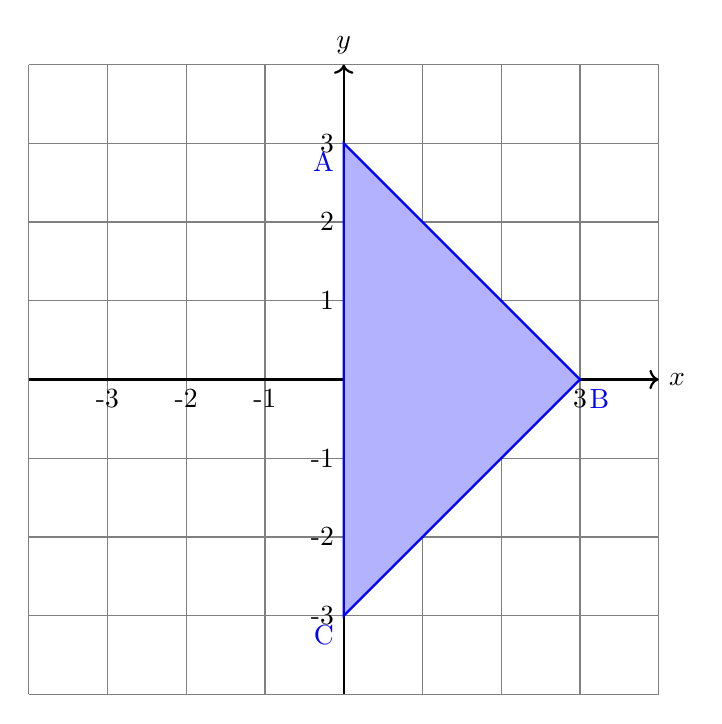
\begin{tikzpicture}
  % Draw grid
  \draw[gray, thin] (-4,-4) grid (4,4);

  % Axes
  \draw[->, thick] (-4,0) -- (4,0) node[right] {$x$};
  \draw[->, thick] (0,-4) -- (0,4) node[above] {$y$};

  % Labels for axes
  \foreach \x in {-3,-2,-1,1,2,3} {
    \node[below] at (\x, 0) {\x};
  }
  \foreach \y in {-3,-2,-1,1,2,3} {
    \node[left] at (0, \y) {\y};
  }

  % Rotated triangle (90 degrees clockwise)
  \fill[blue!30] (0,3) -- (3,0) -- (0,-3) -- cycle; % Fill with blue color, 30% opacity
  \draw[thick, blue] (0,3) -- (3,0) -- (0,-3) -- cycle; % Outline of the triangle
  
  % Vertex labels
  \node[blue] at (0,3) [below left] {A};
  \node[blue] at (3,0) [below right] {B};
  \node[blue] at (0,-3) [below left] {C};
  
\end{tikzpicture}


We have that it is type 1 because for any $(x,y)\in R,$ we have that if $0\leq x \leq 3,$ then there exists smooth functions 
\[g_1(x) = -3 + x, \qquad g_2(x) = 3 -x\] such that $g_1(x)\leq y \leq g_2(x).$\\

However, it is not type 2 because if you take the point $(3,0)\in R,$ it cannot be bounded to the right by a smooth function because of the sharp corner (in fact, any point along $y=0$ works great).
    \end{solution}
\item
\begin{problem}
    Give an example of a region that is neither type 1 nor type 2.
\end{problem}
\begin{solution}
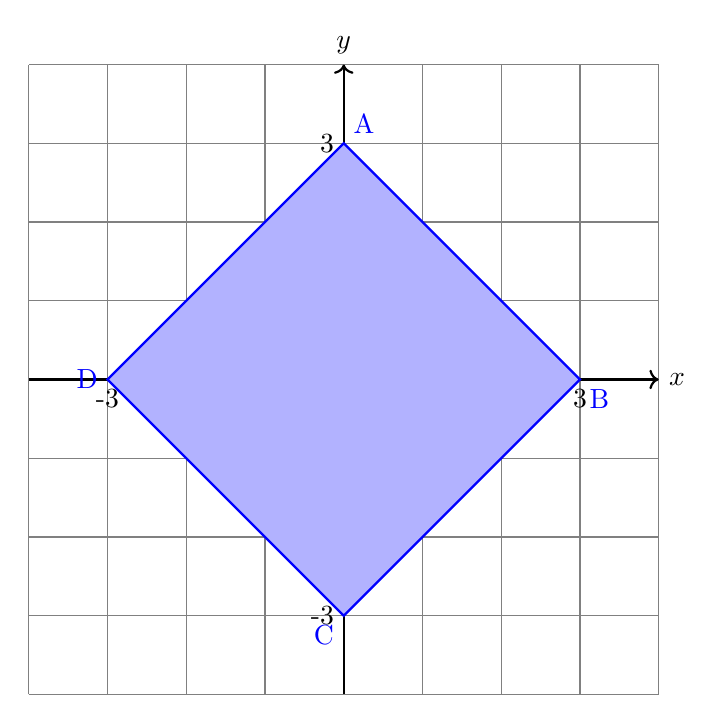
\begin{tikzpicture}
  % Draw grid
  \draw[gray, thin] (-4,-4) grid (4,4);

  % Axes
  \draw[->, thick] (-4,0) -- (4,0) node[right] {$x$};
  \draw[->, thick] (0,-4) -- (0,4) node[above] {$y$};

  % Labels for axes
  \foreach \x in {-3,-2,-1,1,2,3} {
    \node[below] at (\x, 0) {\x};
  }
  \foreach \y in {-3,-2,-1,1,2,3} {
    \node[left] at (0, \y) {\y};
  }

  % Rotated triangle (90 degrees clockwise)
  \fill[blue!30] (-3,0) -- (0,3) -- (3,0) -- (0,-3) -- cycle; % Fill with blue color, 30% opacity
  \draw[thick, blue] (-3,0) -- (0,3) -- (3,0) -- (0,-3) -- cycle; % Outline of the triangle
  
  % Vertex labels
  \node[blue] at (0,3) [above right] {A};
  \node[blue] at (3,0) [below right] {B};
  \node[blue] at (0,-3) [below left] {C};
  \node[blue] at (-3,0) [left] {D};
\end{tikzpicture}

It is clear by the same reasoning as above that this is neither type 1 nor type 2.
\end{solution}
\item 
\begin{problem}
    Is every simple region starlike? convex?
\end{problem}
\begin{solution}
    No consider a function that looks like nearly-headless Nick's moustache as in the Figure below. I apologize for the bad drawing, I am no artist (only consider the moustache curve, not the circle around it or the weird shape intersecting it, that's my bad). We have that this shape is pretty obviously not starlike and thus not convex. To show it is simple, simply split it up into vertical and horizontal lines. Every such line only intersect the curve at a single point (if it doesn't, then that's because I'm bad at drawing). Moreover, every line intersects with a smooth curve (no sharp corners, etc). 
\end{solution}
\begin{figure}[h!]
    \centering
    \includegraphics[width=0.25\linewidth]{Images/7.5.png}
    \caption{Neither starlike nor convex simple region.}
\end{figure}
\item 
\begin{problem}
    If a convex region is bounded by a smooth simple closed curve, is it simple?
\end{problem}
\begin{solution}
    \textbf{Yes.} Let $R$ be such a region. Intuitively, we have that it is bounded by no sharp corners and it does not have any holes or significant dips or dents. We wish to show that if $(x,y)\in R,$ then there exists smooth curves such that $g_1(x)\leq y \leq g_2(x).$ We claim that $C,$ the boundary of $R,$ is such a curve. We have smoothness by assumption. Since $C$ is closed and bounded (since it is closed), then it must be compact, and so it achieves its min/max in the horizontal and its min/max in the vertical. Call the $x$ components of the horizontal min/max $a$ and $b$ and the $y$ components of the vertical directions min/max $c,d.$ Thus, we have that $ R \subset C \subset [a,b]\cross [c,d].$ Thus, we have that $a\leq x \leq b.$ Consider the vertical line across $x.$ Since $C$ is simple, we have that it intersects with $C$ at most twice. Since the curve is smooth, we implicit function theorem to implicitly define the function this vertical line intersects. Since $R$ is convex, we must have that for any $y$ in this vertical line inside the boundary, $y \in R.$ Thus, $y$ is bounded by the smooth curve above and below. This shows that it is Type I. To show it is Type 2, take some $y$ with $c \leq y \leq d,$ then we have that any horizontal line across $y$ intersects with $C$ at most twice, and this if $x$ in the line inside the boundary, $x$ is bounded by the smooth curve to the left and right. Thus, $R$ is Type II.
\end{solution}
\item 
\begin{problem}
    Give an example of a region that divides into three simple subregions but
 not into two.
\end{problem}
\begin{solution}
  
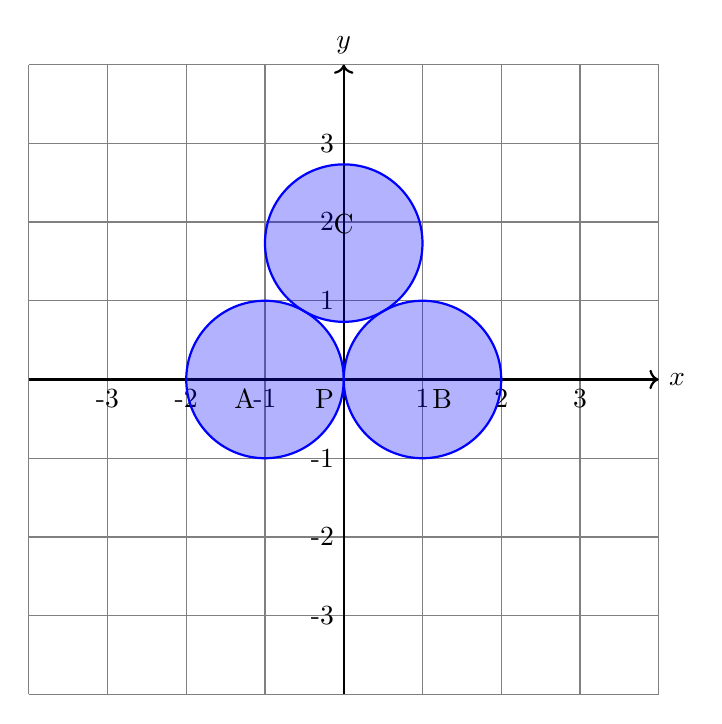
\begin{tikzpicture}
  % Draw grid
  \draw[gray, thin] (-4,-4) grid (4,4);

  % Axes
  \draw[->, thick] (-4,0) -- (4,0) node[right] {$x$};
  \draw[->, thick] (0,-4) -- (0,4) node[above] {$y$};

  % Labels for axes
  \foreach \x in {-3,-2,-1,1,2,3} {
    \node[below] at (\x, 0) {\x};
  }
  \foreach \y in {-3,-2,-1,1,2,3} {
    \node[left] at (0, \y) {\y};
  }

  \fill[blue, opacity=0.3] (-1, 0) circle(1);  % Circle A
  \fill[blue, opacity=0.3] (1, 0) circle(1);  % Circle B
  \fill[blue, opacity=0.3] (0, {sqrt(3)}) circle(1);  % Circle C
  % Draw the three circles
  \draw[thick, blue] (-1, 0) circle(1);  % Circle A
  \draw[thick, blue] (1, 0) circle(1);  % Circle B
  \draw[thick, blue] (0, {sqrt(3)}) circle(1);  % Circle C

  % Labels for the circles
  \node at (-1, 0) [below left] {A};
  \node at (1, 0) [below right] {B};
  \node at (0, {sqrt(3)}) [above] {C};

  % Intersection points (approximated)
  \node at (0, 0) [below left] {P};

\end{tikzpicture}

Here, we have the region of $D = D_1 \cup D_2 \cup D_3,$ where $D_i$ is a disk of radius $1$ intersecting the other $2$ at exactly one point. Evidently, we can split it into $D_1,$ $D_2,$ $D_3,$ each one simple. Evidently, splitting it into two subregions creates at least one region which is not simple, since there do not exist smooth curves to bound anything else than each $D_i.$
\end{solution}
\item 
\begin{problem}
    If a region is bounded by a smooth simple closed curve C then it need not
 divide into a finite number of simple subregions. Find an example.
\end{problem}
\begin{figure}[h!]
        \centering
        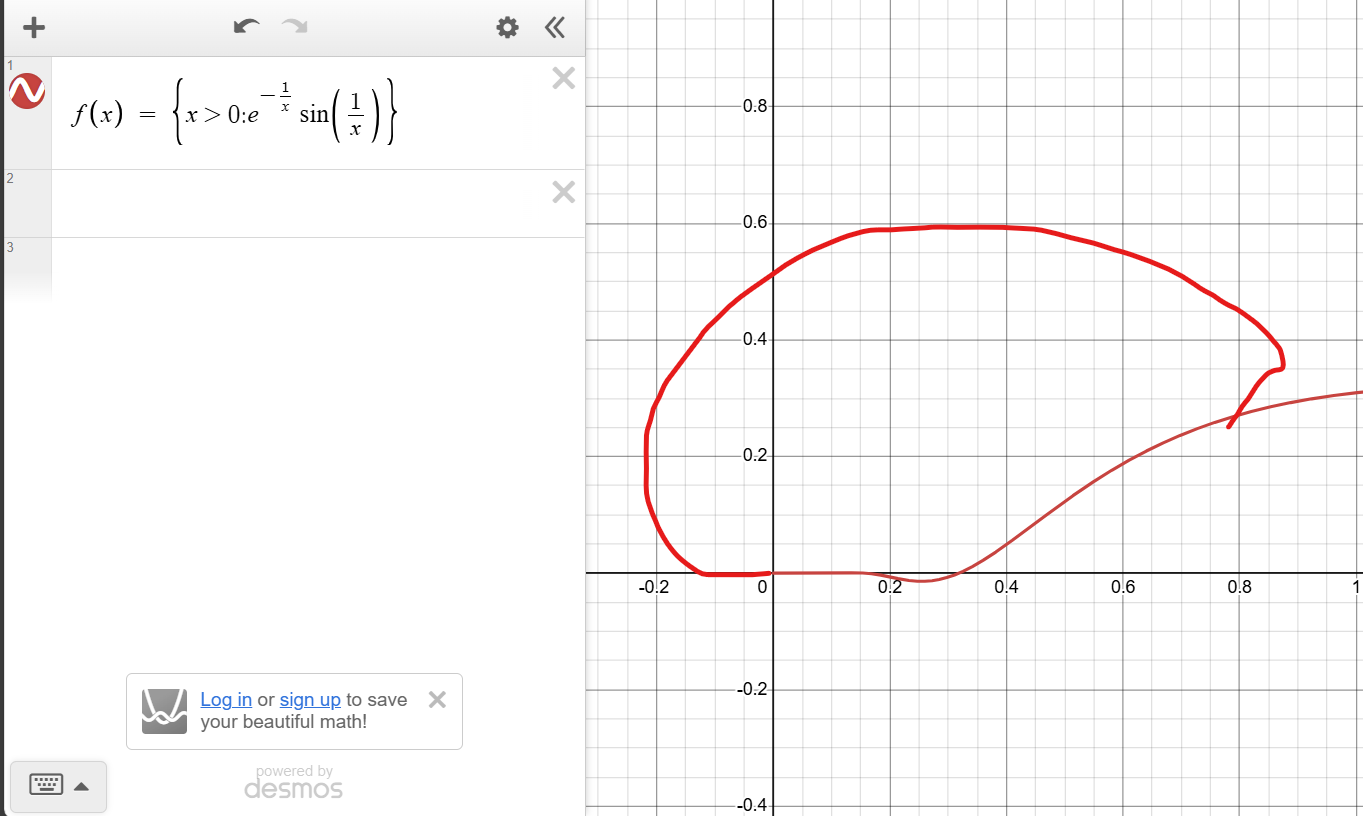
\includegraphics[width=0.5\linewidth]{Images/7.1.png}
        \caption{$e^{\frac{-1}{x}}\sin(\frac{1}{x})$}
    \end{figure}
    \begin{figure}
        \centering
        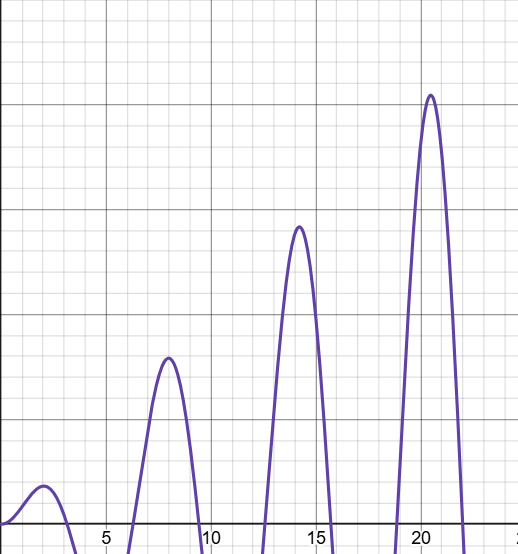
\includegraphics[width=0.25\linewidth]{Images/7.2.png}
        \caption{Some subregion contains bumps like these}
    \end{figure}
\begin{solution}
    Consider the region bounded by the curve
    $f(x) = e^{\frac{-1}{x}}\sin(\frac{1}{x})$ connected at the origin by a smooth curve that goes all the way around to the other end. An image to keep in mind is Figure 2 above. Suppose that it can be divided into a finite number of simple subregions, then near the origin, there must exist some subregion containing more than one bump (in fact, pigeonhole says that it will contain an infinite number of bumps). I.e, we have a subregion bounded below by something like Figure 3 above. This subregion is evidently not Type II though. 
\end{solution}
\item 
\begin{problem}
     Infer that the standard proof of Green’s Formulas for simple regions (as,
 for example, in J. Stewart’s Calculus) does not immediately carry over to
 the general planar region R with smooth boundary; i.e., cutting R into
 simple regions can fail.
\end{problem}
\begin{solution}
    As shown above, it is sometimes impossible to cut a general planar region $R$ into simple regions, and thus his proof does not carry over.
\end{solution}
\item 
\begin{problem}
    Is there a planar region bounded by a smooth simple closed curve such
 that for every linear coordinate system (i.e., a new pair of axes), the region
 does not divide into finitely many simple subregions? In other words, is
 Stewart’s proof of Green’s Theorem doomed?
\end{problem}
\begin{figure}[h]
        \centering
        
\includegraphics[width=0.5\linewidth]{7.3.png}
        \caption{Is Stewart's proof doomed?}
    \end{figure}
\begin{solution}
\textbf{No.} His proof is not doomed. Marrs' proof is aight, but see Desmond's proof for a better one (he stole it from me).
\end{solution}
\item 
\begin{problem}
    Show that if the curve $C$ in (f) is analytic, then no such example exists.
\end{problem}
\begin{solution}
    It suffices to show that if $C$ is analytic, then it cannot have infinitely many bumps around a point. That is, we cannot have a situation as in (f) where there were an infinite number of zeros of the curve that lead up to the origin. We do this by contradiction. That is, suppose that for some $(x,y)\in C,$ we have that for any neighborhood around $(x,y),$ $C$ has infinitely many zeros. It is no loss of generality to call the point the origin and look at the zeros of the curve crossing the $x-$axis. Thus, for any $h>0,$ we have that $C$ intercepts the axis infinitely many times withing $(0,0)$ and $(h,0).$ Since $f$ is analytic, we can express it as 
    \[f(h) = \sum_{k =0}^\infty a_k h^k\] for $h>0$ (suppose further that $|h|< r,$ where $r>0$ is the radius of convergence). By the hint, we have that since $f$ is nonconstant around the origin (since it is smooth then it must be nonconstant since it intersects with the axis infinitely many times), and thus for each $h>0,$ there is some derivative of $f$ which is nonzero. Our contradiction is that $f$ is constantly zero around the origin. Note that we assume that $f(0) = 0,$ implying that $a_0 = 0.$ Consider that as $h\to 0,$ we have that
    \[\lim_{h\to 0}f(h) = \lim_{h\to 0}\left[\sum_{k=0}^\infty a_k h^r\right] = \lim_{h\to 0}\left[a_0 + a_1h + \sum_{k=2}^\infty a_k h^r\right] = 0,\] and so for $h$ small enough, we have that since the series is absolutely convergence for $|h|<r,$ then the tail of the series will still absolutely converge, and thus since $h \to 0,$ we have that
    \[a_1 = -h\sum_{k=2}^\infty a_k h^{r-2} \to 0 \implies a_1 = 0.\] We induct on this process to show that for all $k \in \bbN,$ $a_k = 0.$ Thus, we have that $f(h) \equiv 0$ for $|h|<r,$ but then for any $r \in \bbN$ (sorry for abuse of notation), we have that since all $a_k = 0,$ then
    \[f^{(r)}(h) = \sum_{k=r}^\infty \frac{k!}{(k-r)!}a_k h^{k-r} = 0,\] which is a contradiction to the hint.
\end{solution}
\begin{figure}[h!]
    \centering
    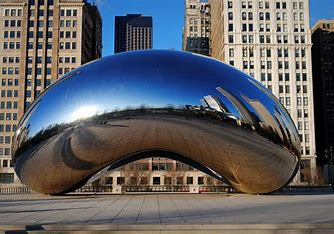
\includegraphics[width=0.5\linewidth]{Images/7.4.png}
    \caption{Jeremy Allen White as a Region that does Not Divide into Two}
\end{figure}
\begin{problem}
    
\end{problem}
\end{enumerate}


\newpage
\section*{Problem 5}
\begin{problem}
    Does there exist a continuous mapping from the circle to itself that has no
 fixed-point? What about the 2-torus? The 2-sphere?
\end{problem}
\begin{solution}
The following maps are all isometries, and are thus continuous.
    \begin{itemize}
        \item (circle) Rotate each point in the circle $180^\circ.$ We have showed in PSET 2 that this map is continuous. It evidently has no fixed point.
        \item (2-torus) For any point on the torus, the point lies along a circle (which would be the cross section of the torus at the point- think of slicing the torus with a knife at the point). Rotate the whole circle $180^\circ$ around the torus. We can also think of this map as just rotating the entire torus around its center $180^\circ.$ 
        \item (2-sphere) map each point in the sphere to be at its anti-pole. This map is continuous for similar reasons to the first. Evidently, there is no fixed point. 
    \end{itemize}
\end{solution}










\end{document}